\documentclass[conference]{IEEEtran}
\IEEEoverridecommandlockouts
% The preceding line is only needed to identify funding in the first footnote. If that is unneeded, please comment it out.
\usepackage{amsmath,amsthm,amssymb} %modos matemáticos y  simbolos
\usepackage{latexsym,amsfonts} %simbolos matematicos
\usepackage{cancel} %hacer la linea que cancela las ecuaciones
\usepackage[spanish, es-noshorthands]{babel} %comandos en español y cambia el cuadro por la tabla
\decimalpoint %cambia las comas por puntos decimal
\usepackage[utf8]{inputenc} %caracteristicas del español
\usepackage{physics} %Simbolos fisicos
\usepackage{array} %mejores formatos de tabla
\parindent =0cm %sangria 
\usepackage{algorithmic}
\usepackage{graphicx}
\usepackage{textcomp}
\usepackage{xcolor}
\usepackage{mathtools} 
\usepackage[framemethod=TikZ]{mdframed}%Entornos talegas
\usepackage[colorlinks = true,
			linkcolor = blue,
			citecolor = black,
			urlcolor = blue]{hyperref}%formato de los links y URL's
\usepackage{multicol} %varias columnas
\usepackage{enumerate} %enumeraciones
\usepackage{pgf,tikz,pgfplots} %documentos en formato tikz
\usepackage{mathrsfs} %letras chingonas (transformada de laplace)
\usepackage{subfigure} %varias figuras seguidas
\usepackage{tabulary}
\usepackage{multirow} %ocupar varias filas en una tabla
\usepackage{fancybox} %recuadros talegas
\usepackage{float} %ubicar graficas
\usepackage{color}
\usepackage{comment}
\usepackage{stackrel}
\usepackage{calligra}
\usepackage{lipsum}
\usepackage{cite}
\pgfplotsset{compat=1.16} 

\newcommand{\R}{\mathbb{R}}
\newcommand{\Z}{\mathbb{Z}}
%%%%%%%%%%%%%%%%%%%%%%%%%%%%%%%%%%%%%%%%%%%%%%%%%%%%%%
\def\BibTeX{{\rm B\kern-.05em{\sc i\kern-.025em b}\kern-.08em
    T\kern-.1667em\lower.7ex\hbox{E}\kern-.125emX}}
    
\usepackage[numbers]{natbib}   

    
\begin{document}

\title{Tarea 1 \\
{\footnotesize \scshape{Mecánica Estadística}}
}

\author{\IEEEauthorblockN{1\textsuperscript{st} Diego Sarceño Ramírez}
\IEEEauthorblockA{\textit{201900109} 
}
%\and
%\IEEEauthorblockN{2\textsuperscript{nd} Andrés Pérez}
%\IEEEauthorblockA{\textit{201704199}
%}
}



\maketitle

%\begin{abstract}
%
%\end{abstract}

%\begin{IEEEkeywords}
%Semáforo, intersección, Flip Flop, tipo D, 555, integrados, compuertas lógicas.
%\end{IEEEkeywords}

\section{Fórmula de Stirling}
La función factorial tiene varias formas de definirse, las que más me gustan son las dos siguientes
	\begin{equation}
		\begin{array}{c}
			n! = \displaystyle\prod _{k = 1} ^n k \\
			n! = \left\{\begin{array}{lr}
				1 & \text{si } n < 2 \\
				(n - 1)! \cdot n & \text{si } n > 1.
			\end{array}\right.
		\end{array}
	\end{equation}
	La productoria y la fórmula de recurrencia. Una forma de aproximar la función factorial es la fórmula de stirling. La aproximación de stirling la deducimos aplicando la función logaritmo a la definición clásica de factorial y, por propiedades de los logaritmos, se separan en sumas:
	\begin{equation*}
		\ln{n!} = \sum _{k = 1} ^n \ln{k} .
	\end{equation*}
	Dado esto, utilizamos la definición de integral en sumatoria, con lo que, desarrollando la integral de $\ln{k}$. Dada esta comparación, es claro que el área bajo la curva dada por la integral es menor a la dada por la sumatoria. Con esto y la solución de la integral
	\begin{equation*}
		\ln{n!} > n\ln{n} - n + 1,
	\end{equation*}
	Esa es una forma de llegar a la fórmula de Stirling; sin embargo, una forma más directa de llegar es por medio de la función gamma, la cual es otra forma de definir la función factorial. Tomando la función gamma y sustituyendo $x^n = e^{n\ln{x}}$, entonces
		$$\Gamma (n) = \int _{0} ^\infty e^{n\ln{x} - x} \dd{x}.$$
	Con esto, realizamos la sustitución $x = n + y$ y $\dd{x} = \dd{y}$, realizando un poco de álgebra en el exponente y sabiendo la serie de Laurent de $\ln{\qty(a + \frac{y}{n})}$, con esto se llega a 
		$$n! \approx e^{-n} n^n \int _{-n} ^{\infty} e^{-\frac{y^2}{2n}} \dd{y}.$$
	Lo que es igual a
		\begin{equation}
			\boxed{n! \approx \sqrt{2\pi n} e^{-n} n^n}
		\end{equation}
\section{Triángulo de Pascal}
\paragraph{Teorema de Construcción del Triangulo de Pascal \cite{freund}} Para todo $n \in \mathbb{Z} ^+$  y $r = 1,2,\ldots ,n-1$, se tiene
	\begin{equation}
		\mqty(n \\ r) = \mqty(n - 1 \\ r) + \mqty(n - 1 \\ r - 1). \label{PascalTriangle}
	\end{equation}

\begin{proof}
	Tomando el teorema del binomio
		\begin{equation}
			(x + y)^n = \sum _{r = 0} ^n \mqty(n \\ r) x^{n - r} y^r ,
		\end{equation}
	si $x = 1$ y expresamos lo restante como $(1 + y)^n = (1 + y) (1 + y) ^{n - 1} = (1 + y) ^{n - 1} + y(1 + y)^{n - 1}$. Con esto encontramos el coeficiente de $y^r$ en los tres términos dados, lo que nos dá
		\begin{equation*}
			\mqty(n \\ r) = \mqty(n - 1 \\ r) + \mqty(n - 1 \\ r - 1),
		\end{equation*}
	lo que justamente es \eqref{PascalTriangle}.
\end{proof}

\paragraph{Visualización} 
La ecuación \eqref{PascalTriangle}, visualmente se representa como
	
\begin{figure}[H]
	\centering
	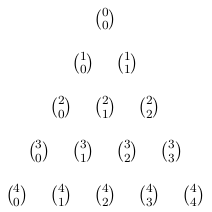
\includegraphics[scale=0.8]{img/triangulo.png}
	\caption{Representación visual del triángulo de pascal. Es claro que cada término de las filas es creado por la suma de los dos superiores.}
	\label{VisualPascalTriangle}
\end{figure}

\section{Gases Ideales}
Los experimentos en gases muestran que la presión ($p$) de un volumen ($V$) de un gas, dependen de su temperatura ($T$). Vease \cite{blundell}.
\subsection{Ley de Boyle}
Dado un gas a temperatura constante, se tiene
	\begin{equation}
		p \propto \frac{1}{V} .\label{BoyleLaw}
	\end{equation}
	
\subsection{Ley de Gay-Lussac}
Para un gas a volumen constante
	\begin{equation}
		p \propto T. \label{GayLussacLaw}
	\end{equation}
\subsection{Charles}
Para un gas a presión constante, se tiene
	\begin{equation}
		V \propto T, \label{CharlesLaw}
	\end{equation}
con $T$ medido en Kelvin.
\subsection{Ley de los Gases Ideales}
Estas tres leyes combinadas forman la ley de gases ideales
	\begin{equation}
		pV \propto T, \label{LawsCombined}
	\end{equation}
para $N$ moleculas en el gas, la expresión anterior se convierte en
	\begin{equation}
		pV = Nk_B T. \label{IdealGas}		
	\end{equation}
\subsection{Constantes}
En la ecuación \eqref{IdealGas}, se introducen dos constantes, la constante de Boltzmann y el Número de Avogadro. 
	\begin{itemize}
		\item {\bf Constante de los Gases Ideales: } Esta constante nace en la teoría de los gases; sin embargo, aparece en ámbitos que no tienen que ver con gases, esto es por como está construída
			\begin{equation}
				R = k_B N_A .\label{constGasIdeales}
			\end{equation}
		Tiene un valor de $R = 8.3144 \flatfrac{J}{\text{mol} \cdot K}$ en el sistema internacional.
		\item {\bf Constante de Boltzmann: } Esta constante relaciona la temperatura absoluta y la energía, recae su importancia en la definición de entropía. Su valor numérico es $k_B = 1.380649 \times 10 ^{23} \flatfrac{J}{K}$, en el sistema internacional.
	\end{itemize}
\subsubsection{Número de Avogadro y Ley de Avogadro}
El número de Avogadro es el factor de proporcionalidad entre el número de partículas o entidades elementales y la cantidad de sustancia. La constante de Avogadro tiene un valor de $N_A = 6.02214076 \times 10^23 \text{mol} ^{-1}$. La ley de avogadro relaciona el nuevo conepto de cantidad de sustancia con el número de partículas para distintas sustancias gaseosas, citando literalmente de \textit{wikipedia} \cite{wiki}: \\	
{\it "Volúmenes iguales de distintas sustancias gaseosas, medidos en las mismas condiciones de presión y temperatura, contienen el mismo número de moléculas."} \\
En otras palabras
	\begin{equation}
		N\propto n, \label{AvogadroLaw}
	\end{equation}
	con $N$ el número de partículas y $n$ el número de moles.
\subsection{Amadeo Avogadro}
Un Físico y Químico italiano, nacido en Italia en $1776$ y fallecido en $1856$. Graduado en $1792$ de doctor en derecho canónico. En $1809$, obtiene el puesto de profesor en el colegio real de Vercelli, en $1811$, enunció la hipótesis de la, ahora conocida, ley de Avogadro. Para ello se apoyó en la teoría atómiac de Dalton y el la ley de Gay-Lussac, \eqref{GayLussacLaw}. En $1814$ publicó un trabajo llamado "Memoria sobre las masas relativas de las moléculas de los cuerpos simples, o densidades esperadas de su gas, y sobre la constitución de algunos de sus compuestos, para servir seguidamente como ensayo sobre el mismo sujeto", y en $1820$ publicó otro llamado "Nuevas consideraciones sobre la teoría de las proporciones determinadas en las combinaciones, y sobre la determinación de las masas de las moléculas de los cuerpos" y poco después "Memoria sobre la forma de incluir los compuestos orgánicos en las leyes ordinarias de las proporciones determinadas". En el año $1820$, la universidad de Turín creó una cátedra para él, la cual ocuparía hasta su muerte.
\subsection{Ludwig Boltzmann}
Un físico austríaco nacido en Viena en el año $1844$ y fallecido en $1906$. Un pionero en Mecánica Estadística, graduado de doctor de la universidad de Viena en $1866$. Trabajó como docente en la Universidad de Viena por el año de $1894$, y en $1900$ se traslado a Leipzig. Entre sus obras más reconocidas están las que fueron publicadas en $1870$ en las cuales expone cómo la segunda ley de la termodinámica se puede explicar aplicando análisis estadísiticos, de donde deduce el teorema de equipartición de la energía y derivó una ecuación para el cambio en la distribución de energía entre los átomos de un sistema debido a las colisiones. A partir de ello realizó nuevos descubrimientos, de los cuales, uno de los más reelevantes es la famosa ecuación de entroía, la cual relaciona estados macroscópicos y microscópicos $S = k_B \ln{\Omega}$. Se suicidó en $1906$.

\bibliographystyle{apalike} 
\bibliography{bibliografia.bib}

\end{document}


